\section{Derivations}
\label{app:proofs}

\paragraph{Proposition~\ref{prop:memo}.}
With non-repeating contexts, the empirical loss of a conditional generator decomposes over training contexts. For the memorizing solution every candidate equals the realized mode, so the minimum distance is zero for every context. For the generalizing solution the candidates are $m$ i.i.d.\ draws from $p(\cdot\,|\,c_i)$, and the realized mode is itself a draw from $p$, so the expected minimum distance is $I(m)$ of Equation~\ref{eq:I}. The difference of the two empirical risks is therefore $I(m)$ in expectation over the realized modes. For the bounds, let the modes be equiprobable with pairwise distances in $[\delta, \Delta]$. The probability that none of the $m$ draws equals the realized mode $k$ is $(1 - 1/K)^m$; on that event the nearest draw is at squared distance in $[\delta^2, \Delta^2]$, and otherwise the distance is zero, which gives the stated bounds. If the modes densely fill a curve of length $\ell$ ($K \gg m$), the draws are $m$ uniform points on the curve and the expected squared arc distance from a uniform point to its nearest draw is $\Theta(\ell^2/m^2)$, as for the nearest of $m$ uniform points on an interval, so $I(m)$ decays polynomially and does not depend on $K$. For squared-error regression the single prediction can memorize the realized mode at zero loss, and the generalizing prediction (the conditional mean) has loss $\mathrm{tr}\,\mathrm{Cov}_p$, independent of any budget. A detail used in Section~\ref{sec:collapse}: the memorization index $s$ is related to the excess memorization by $s = 1/K + (1 - 1/K)\,\mathrm{excess}$, so a $\pm 2$ RMSE interval on the excess scale maps to $\pm 2(1 - 1/K)\,\mathrm{RMSE}$ on the index scale.

\paragraph{Proposition~\ref{prop:shrink}.}
Write $Y_j - X = (\mu - X) + s\,\varepsilon_j$ with $\varepsilon_j \sim \mathcal{N}(0, I_d)$ and $X - \mu \sim \mathcal{N}(0, \sigma^2 I_d)$. Then $\|Y_j - X\|^2 = \|X - \mu\|^2 + s^2 \|\varepsilon_j\|^2 - 2 s\, \varepsilon_j^\top (X - \mu)$. The first term is common to all $j$; the second concentrates at $s^2 d$ with fluctuations of order $s^2 \sqrt{d}$; the third is, conditionally on $X$, Gaussian with variance $4 s^2 \|X - \mu\|^2 \approx 4 s^2 \sigma^2 d$ and independent across $j$, so the minimum over $j$ of the sum is, to leading order in $d$, $d\sigma^2 + d s^2 - 2 s \sigma \sqrt{d}\, e_m$ with $e_m = \E \max_{j \le m} \xi_j$. Minimizing in $s$ gives $s^\star = \sigma e_m / \sqrt{d}$. The spread-to-error ratio used in Section~\ref{sec:bair}, defined as the mean pairwise distance among samples divided by the mean distance from samples to the realized outcome, is $r = \sqrt{2}\rho/\sqrt{1 + \rho^2}$ with $\rho = s/\sigma$ under this model, which is how $\deff$ is fitted from one measured $r$.

\paragraph{Flattening.}
Let the generator place mass $q_k$ on mode $k$ and let all modes be at mutual distance $\Delta$. The probability that none of $m$ draws lands on the realized mode $k$ is $(1 - q_k)^m$, so $L(q) = \Delta^2 \sum_k p_k (1 - q_k)^m$. Minimizing subject to $\sum_k q_k = 1$ gives the stationarity condition $m\, p_k (1 - q_k)^{m-1} = \lambda$ for every $k$ with $q_k > 0$, which is Theorem~7 of \citet{bennett2026freedom}; for $K = 2$ it reads $\big((1-q)/q\big)^{m-1} = (1-p)/p$. If $p_k = 1/K$ for all $k$ the symmetric point $q_k = 1/K$ satisfies the condition and is the unique minimizer of the convex objective for $m \ge 2$ (Theorem~4 of the same work). The numerical optima quoted in the text (for $p = (0.787, 0.213)$: $0.787$, $0.607$, $0.522$ at $m = 2, 4, 16$) solve this equation.

\paragraph{Proposition~\ref{prop:es}.}
(a) The energy distance between $q$ and $\delta_x$ is $2\E_{Y \sim q}\|Y - x\|^\beta - \E_{Y, Y' \sim q}\|Y - Y'\|^\beta - 0$, so $\IS_\beta(q, x)$ is half of it; for $\beta \in (0, 2)$ the energy distance is non-negative and zero only when the two distributions coincide (its square root is a metric on distributions with finite $\beta$-th moments; \citealp{gneiting2007strictly,dawid2007geometry}), so it vanishes only at $q = \delta_x$. The empirical risk over training contexts is a sum of such terms with one $x$ per context, so its unique minimizer is the memorizing solution; the $m$-sample estimator with the unbiased pairwise term has this risk as its expectation for every $m \ge 2$. (b) At $q = p$, $\E_{x \sim p}\,\IS_\beta(p, x) = \E\|Y - x\|^\beta - \frac{1}{2}\E\|Y - Y'\|^\beta = \frac{1}{2}\E\|Y - Y'\|^\beta$ because $x$ and $Y$ are exchangeable. (c) For $\beta = 2$, $\E\|Y - x\|^2 - \frac{1}{2}\E\|Y - Y'\|^2 = \|\E Y - x\|^2$. (d) The per-token score is a sum over tokens of energy scores of the token marginals, and (a)--(b) apply to each term.

\paragraph{Direction insensitivity (interpretation).}
Suppose the generator's mean is offset from the outcome by an unknown vector of length $a$ and it adds isotropic noise of scale $s$ in $d$ dimensions with $d$ large. Then $\E\|Y - x\|^\beta \approx (a^2 + s^2)^{\beta/2}$ and $\E\|Y - Y'\|^\beta \approx (2 s^2)^{\beta/2}$, and the energy score $(a^2 + s^2)^{\beta/2} - \frac{1}{2}(2s^2)^{\beta/2}$ is minimized at $s = a$ for every $\beta \in (0, 2)$, where it equals $2^{\beta/2 - 1} a^\beta$; this is the $\lambda = 1$ case of Proposition~4.1 of \citet{debortoli2025distributional}, and the gain does not depend on $d$. The same calculation for the \nom{} loss follows Proposition~\ref{prop:shrink} and gives $s \approx a\, e_m/\sqrt{d}$. The approximation requires the bias and the noise to be spread over many dimensions (participation ratio $\gg 1$); the regression residual on BAIR has participation ratio about $1{,}030$, and we did not measure it on the bounce tokens. The argument says nothing about where the isotropic spread points; the claim in Section~\ref{sec:es} that it points off the manifold is an empirical observation.

\FloatBarrier
\section{$I(m,K)$ for the bounce geometry and the recorded predictions}
\label{app:pred}
\label{app:imk}
At a wall frame the $K$ possible next directions are the unit vectors at angles $\theta_k = \big((k + \tfrac12)/K\big)\,180^\circ - 90^\circ$ about the wall normal, $k = 0, \dots, K-1$, with unit speed. For a target mode $k$ let $d^{(k)}_{(1)} \le \dots \le d^{(k)}_{(K)}$ be the sorted squared distances from $\mu_k$ to all modes ($d^{(k)}_{(1)} = 0$). The nearest of $m$ i.i.d.\ uniform draws is the $r$-th closest mode with probability $\big((K - r + 1)/K\big)^m - \big((K - r)/K\big)^m$, so
\begin{equation}
I(m, K) = \frac{1}{K} \sum_{k=1}^{K} \sum_{r=1}^{K} d^{(k)}_{(r)} \Big[ \big(\tfrac{K - r + 1}{K}\big)^m - \big(\tfrac{K - r}{K}\big)^m \Big].
\end{equation}
\paragraph{Predictions tested in the paper.} P1: excess memorization falls on one curve across $K$ against $I(m,K)$, not against $(1-1/K)^m$ ($K \in \{2,16\}$ values recorded in advance; Section~\ref{sec:collapse}). P2: the energy score memorizes in non-repeating contexts at every $m$, faster at larger $m$, and stops when contexts carry no identifying feature (derived after the first energy-score runs; the follow-up predictions were recorded in advance; Section~\ref{sec:es}). P3: with $p = (0.8, 0.2)$ the frequent-mode share of \imlewm{} samples falls with $m$ as prescribed (shares recorded in advance without a tolerance; Section~\ref{sec:flatten}). P4: on real video the spread grows with $m$ only like $e_m$ and $m{=}64$ does not reach FM-50's distribution metrics (fitted after the BAIR runs; the recorded parameter-free version failed; Section~\ref{sec:bair}). P5: the energy score's spread is off-manifold, so its deficit survives a noise-robust readout (not recorded in advance; Section~\ref{sec:es}).

\paragraph{Predictions recorded before the runs.} The following predictions were written into dated notes or run scripts before we saw the results of the corresponding runs; these records are our own and are not externally timestamped. (i) The nine memorization indices for $K \in \{2, 16\}$ of Table~\ref{tab:predfull}; seven fell inside their intervals. (ii) For the asymmetric variant, frequent-mode shares of $0.80$, $0.61$ and $0.52$ for \imlewm{} with $m = 2$, $4$, $16$ and of about $0.80$ for flow matching, computed for the nominal $p = 0.8$, without a tolerance; the measured shares are $0.82$, $0.65$, $0.57$ and $0.83$ (Table~\ref{tab:flatten}), and the comparison relative to FM-50 used in Section~\ref{sec:flatten} was chosen after the runs. (iii) Five predictions for the energy-score follow-up runs (P1--P5 of Appendix~\ref{app:es}) and two for their second seeds (the energy score with $m{=}16$ again reaches an index of at least $0.87$ and a coverage of at most $0.36$, observed $0.97$ and $0.29$; P1--P3 hold again); all seven held. (iv) Three predictions for the fed-back-state ablation (S1--S3, Appendix~\ref{app:seq}); all held. (v) On BAIR, that the participation ratio of the regression residuals lies within a factor of two of the value of $d$ fitted at the time ($29$, i.e.\ $14.5$--$58$), and that Proposition~\ref{prop:shrink} with this $d$ predicts the spread-to-error ratios at $m = 4$, $16$, $64$ within $0.10$; both failed (about $1{,}030$; predicted ratios $0.05$--$0.10$ against measured $0.22$--$0.54$). After this failure we designed an exploratory analysis with four recorded predictions: the per-context participation ratio of the samples is at most a fifth of that of the residuals (held); with $d$ set to it, Proposition~\ref{prop:shrink} predicts the $m{=}16$ ratio within $0.10$ (failed: $1.12$ against $0.45$); it changes by less than a factor of two from $m{=}4$ to $m{=}64$ (failed narrowly: $1.18$ to $2.52$); and the sample directions capture more of their own context's residual than of another context's (held). In total 17 of the 21 predictions with a tolerance held, and 2 of the 4 exploratory ones.

\paragraph{Recorded predictions for the $K{=}2,16$ grid.} Table~\ref{tab:predfull} lists the values together with the predictions recorded before the $K \in \{2, 16\}$ runs. The predictions were made by fitting excess memorization linearly in $I$ on the eight $K \in \{4, 8\}$ points (excess $= 0.015 + 1.06\,I$, RMSE $0.032$) and mapping to the index scale; the intervals are $\pm 2$ RMSE. We noted two risks at the time: the $K{=}2$, $m{=}2$ point lies outside the fitted range of $I$, and large $K$ might memorize less than predicted because more bits must be stored per context. Both failures are of these kinds.

\begin{table}[h]
\caption{Recorded predictions for the memorization index at 8k steps and the observed two-seed means. The two failed predictions are marked.}
\label{tab:predfull}
\begin{center}
\small
\resizebox{\linewidth}{!}{%
\begin{tabular}{cccccc}
\toprule
$K$ & $m$ & $I(m,K)$ & Chance & Predicted [interval] & Observed \\
\midrule
2 & 2 & 0.500 & 0.50 & 0.77 [0.74, 0.81] & 0.956 (failed) \\
2 & 4 & 0.125 & 0.50 & 0.57 [0.54, 0.61] & 0.568 \\
2 & 8 & 0.008 & 0.50 & 0.51 [0.50, 0.54] & 0.528 \\
2 & 16 & $\approx 0$ & 0.50 & 0.51 [0.50, 0.54] & 0.522 \\
16 & 4 & 0.234 & 0.0625 & 0.31 [0.25, 0.37] & 0.221 (failed) \\
16 & 8 & 0.074 & 0.0625 & 0.15 [0.09, 0.21] & 0.144 \\
16 & 16 & 0.021 & 0.0625 & 0.10 [0.06, 0.16] & 0.115 \\
16 & 32 & 0.005 & 0.0625 & 0.08 [0.06, 0.14] & 0.105 \\
16 & 64 & 0.0006 & 0.0625 & 0.08 [0.06, 0.14] & 0.081 \\
\midrule
4 & 4 / 8 / 16 / 32 & 0.235 / 0.061 / 0.006 / 0.0001 & 0.25 & (fitted) & 0.498 / 0.306 / 0.272 / 0.263 \\
8 & 4 / 8 / 16 / 32 & 0.236 / 0.076 / 0.019 / 0.002 & 0.125 & (fitted) & 0.305 / 0.198 / 0.154 / 0.144 \\
\bottomrule
\end{tabular}}
\end{center}
\end{table}

\FloatBarrier
\section{Benchmark construction}
\label{app:bench}

\paragraph{A2 appearance randomization.}
Each episode of A2-div draws a 22-dimensional appearance vector: background RGB in $[10, 110]$, ball RGB in $[150, 255]$, radius in $[3, 6]$\,px, speed in $[10, 18]$\,px per frame, and two rectangles with top-left corner coordinates in $[0, 48]$, side lengths in $[6, 20]$ and RGB in $[40, 200]$. Frames are rendered at $64\times64$ with an anti-aliased disc, upsampled to $224$\,px and encoded by DINOv2 ViT-S/14. Context novelty is the ratio between the median distance from a test context to its nearest training context and the median nearest-neighbor distance within the training set, both measured in a PCA-64 token space: $1.9$ for A2-div and $0.35$ for A2-fix. The evaluation uses 400 held-out wall contexts; a stochastic transition is one whose current frame touches a wall.

\paragraph{Push environment.}
The $64\times64$ arena contains an ice rectangle ($x \in [20, 44]$, $y \in [14, 40]$) and an absorbing pit ($x \in [24, 40]$, $y \in [0, 14]$). A push action is a 2-D vector; with probability $0.1$ it is zero, and otherwise its direction is uniform and its magnitude is uniform in $[0.3, 1]$. The ball moves $10$\,px along the action direction rotated by the sampled deflection, and it respawns after four frames in the pit. The branch-risk task draws starting positions with $x \in [8, 12]$, $y \in [17, 21]$ and goals with $x \in [52, 56]$ in the same $y$ band. The planner uses CEM-MPC with horizon $T{=}5$, 64 candidate sequences, $m_p{=}8$ imagined futures per candidate (one for regression), and a cost equal to the mean distance between the decoded final position and the goal; 100 episodes per model and seed with a shared set of task seeds. The risk diagnostic evaluates 200 start states with the straight five-push action sequence against 256 true-simulator rollouts per start, and a one-push test from 200 ice states just below the pit.

\paragraph{Stochastic Push-T hidden variable.}
Table~\ref{tab:cog} shows the per-episode randomizations we tried before choosing the center of gravity; mass and friction have no effect under Push-T's quasi-static physics, and damping produces unrealistic sliding. The multi-future test set takes 128 starting states just before the first contact (an earlier version with starts further from contact did not diverge within 8 steps and was discarded), and for each start the 64 futures share the three context frames. Modes closer than $2$\,px in outcome are merged, leaving $4.0$ distinguishable modes per start on average ($3.99$ at $h{=}8$). The CEM planner for Push-T uses $T{=}5$, 64 candidates, $m_p{=}4$, 3 iterations with 8 elites, re-planning every step for at most 10 steps, with the mean token-space $\ell_2$ distance to the goal as the cost, following \citet{terver2025drives}; goals are within 25 steps of the start, and success requires the block within $20$\,px and $20^\circ$ of the goal.

\begin{table}[h]
\caption{Candidate hidden variables for stochastic Push-T: deviation of the T vertices after 16 steps under the same actions (median / maximum over episodes; the nominal displacement is $124$\,px).}
\label{tab:cog}
\begin{center}
\small
\begin{tabular}{lcl}
\toprule
Randomization & Deviation (px) & Decision \\
\midrule
Block mass $0.5$--$2\times$ & 0.0 / 0.0 & no effect (quasi-static) \\
Contact friction $0.3$--$1.2$ & 0.0 / 0.0 & no effect \\
Damping $0$--$0.1$ & 25 / 346 & unrealistic sliding \\
Center of gravity, radius $20$\,px, 4 positions + 3\,px jitter & 28 / 138 & adopted \\
Center of gravity, radius $25$\,px & 56 / 195 & too large \\
\bottomrule
\end{tabular}
\end{center}
\end{table}

\paragraph{BAIR.}
We use the first part of the official archive: $4{,}096$ training sequences and $1{,}024$ held-out sequences (the official test set plus three held-out training files), $64\times64$ frames, 4-dimensional actions, 3 context frames and 16-step rollouts.

\FloatBarrier
\section{Implementation details and ablations}
\label{app:impl}
Code, environments, the queue files that define every run and the per-run outputs behind every figure and table will be released with the paper.

\paragraph{Training.}
AdamW with learning rate $2\times10^{-4}$, $(\beta_1, \beta_2) = (0.9, 0.9)$, no weight decay, a linear warm-up over 1{,}000 steps followed by a cosine decay, batch 128, gradient clipping at norm 1, an exponential moving average (EMA) of the weights with decay $\min(0.999, (1 + t)/(10 + t))$ used for all evaluations, 12k steps (8k for the budget grid, the asymmetric variant and the per-step-matching comparisons; 36k for iMF; 24k for Shortcut; 48k for the four-times-longer A1 runs). The noise vector has 256 dimensions and is normalized to unit RMS before the mapping network. Late fusion sets the first five of eight blocks (eight of twelve for the 21M model) to a learned constant style. Candidate generation for matching runs without gradient tracking, in bfloat16, in a separate autocast region; if it shares a region with the gradient pass, autocast reuses the weight casts made without gradient tracking and silently cuts the gradient to the weights. The Geman--McClure scale is twice the running median (EMA $0.99$) of the matching distance. The energy-score runs use $\beta = 1$, the whole-map RMS distance, the unbiased pairwise estimator, and backpropagate in two chunks of contexts; the per-token variant computes pairwise differences explicitly to be exact near zero. Flow matching uses the time shift $\alpha = 13$ at training and sampling and the Euler sampler. The iMF port follows the official JAX implementation through a PyTorch re-implementation: dual $u$/$v$ heads of width 640 (to match parameters), the Jacobian--vector-product (JVP) direction taken from the model's own $v$ prediction, and the loss $\|u + (t - r)\,\mathrm{sg}(\partial_t u) - v\|^2$ with $\mathrm{sg}$ the stop-gradient, plus a flow-matching loss on $v$; it converges only with the time-embedding frequency scale set to 1 rather than the usual 1000. Our own earlier MeanFlow implementation diverged in three attempts once the average-velocity term was switched on, and was abandoned. Shortcut models devote a quarter of each batch to the self-consistency target computed with the EMA model. Parameter counts: 8M setting, $7.97$--$8.24$M across methods ($8.24$M for \imlewm{}); 21M setting, $20.6$M for \imlewm{}. Training times in the tables are wall-clock hours on one RTX A5000; some runs shared a GPU and are therefore slower than the stand-alone timings (one training step at batch 128: 178\,ms for $m{=}4$ and 488\,ms for $m{=}16$ with the 8M model; 404 and 1112\,ms with the 21M model).

\paragraph{Recipe choices.}
Table~\ref{tab:recipe} gives the pilot comparisons behind the recipe. The wide head does not change \imlewm{}'s results (it is there to match the flow baselines); late fusion halves training time at equal coverage and lowers the deterministic-transition error; the FlowWM recipe raised the flow baseline substantially. Multi-stage supervision, which ROMS-IMLE found important for images, does not help on a fixed $16\times16$ token grid (Appendix~\ref{app:negative}).

\begin{table}[h]
\caption{Recipe comparisons on A2-div ($K{=}4$, pilot and preparation runs, one seed). Intervals are bootstrap 95\% intervals over the 300 held-out contexts of the memorization monitor (400 evaluation contexts for the default-recipe FM row). The monitor samples the flow models with 20 Euler steps, so the coverage and precision of the iMF row are 20-step values (its deterministic-transition error is a one-step value). Training hours are on a shared GPU.}
\label{tab:recipe}
\begin{center}
\small
\resizebox{\linewidth}{!}{%
\begin{tabular}{lcccccc}
\toprule
Variant & Coverage & Precision & kNN recall & Det.\ err.\ (px) & Memo.\ (train / held-out) & Train (h) \\
\midrule
\imlewm{} $m{=}16$, full noise injection, wide head & 0.934 [0.917, 0.949] & 0.83 & 0.94 & 2.31 & 0.29 / 0.24 & 1.93 \\
\imlewm{} $m{=}16$, late fusion, wide head (adopted) & 0.925 [0.907, 0.942] & 0.83 & 0.95 & 1.56 & 0.29 / 0.27 & 1.05 \\
\imlewm{} $m{=}16$, full injection, narrow head (6.6M) & 0.930 [0.909, 0.948] & 0.84 & 0.94 & 2.02 & 0.30 / 0.25 & 1.71 \\
\imlewm{} $m{=}16$, pilot recipe (three spatial stages) & 0.91 [0.89, 0.93] & 0.81 & 0.94 & 2.67 & 0.30 / 0.22 & 3.2 \\
FM, default recipe, 20 Euler steps & 0.58 [0.55, 0.61] & 0.38 & 0.68 & 4.64 & -- & 0.6 \\
FM, FlowWM recipe, 50 steps (adopted) & 0.79 [0.77, 0.82] & 0.51 & 0.91 & 2.27 & 0.29 / 0.24 & 0.4 \\
iMF, time-embedding scale 1000 & \multicolumn{5}{c}{does not converge} \\
iMF, time-embedding scale 1, 12k steps & 0.55 [0.52, 0.58] & 0.22 & -- & 13.1 & -- & 1.0 \\
\bottomrule
\end{tabular}}
\end{center}
\end{table}

\paragraph{Ablations.}
\label{app:ablation}
On A2-div with $m{=}16$ (one seed): replacing Geman--McClure by $\ell_2$ gives coverage $0.93$, precision $0.83$, index $0.28$, deterministic-transition error $1.81$\,px (vs.\ $1.55$); a 64-dimensional noise vector gives $0.92$, $0.83$, $0.28$, $1.50$; training $1.5\times$ longer (18k steps) gives $0.92$, $0.86$, $0.31$, $1.45$. On stochastic Push-T an 8M \imlewm{} with $m{=}16$ reaches recall errors $24.5$ / $39.0$\,px at $h = 8$ / $16$ against $22.1$ / $37.8$ for the 21M model (three seeds), so model size matters little there. In the pilot with the earlier recipe, Geman--McClure improved precision ($0.92$ vs.\ $0.86$) and token-space coverage ($0.85$ vs.\ $0.66$) over $\ell_2$. The iMF learning curve on A2-div (one seed, checkpoints of a 72k-step run) saturates after 24k steps: coverage $0.56$, $0.57$, $0.58$, $0.58$ and precision $0.24$, $0.25$, $0.26$, $0.26$ at 24k, 42k, 60k and 72k steps.

\FloatBarrier
\section{Readouts}
\label{app:readout}
Position readouts are small networks trained on real tokens: a soft-argmax probe for the ball (test error $0.13$\,px on A2-div, $0.05$\,px with DINOv3 on A1), and for Push-T a probe for agent position, block position and angle (T-vertex error $2.0$\,px). Because a probe might decode generated (out-of-distribution) tokens differently from real ones, the pilot cross-checked it against a nearest-neighbor judge that decodes a token map by looking up the nearest of $12{,}000$ real frames in a PCA-128 space: on the fixed-appearance environment the two judges agreed within $0.01$ for every \imlewm{} run (e.g.\ coverage $0.960$ vs.\ $0.960$ at $K{=}4$) and the nearest-neighbor judge was $0.03$--$0.09$ lower for flow matching ($0.841$ vs.\ $0.814$ with 20 steps), so the probe is, if anything, generous to the baselines; the ranking was identical under both. The FlowWM heatmap readout, ported from the public code, maps the $384$-channel token map through a $1\times1$ convolution to 256 channels, a GELU, dropout $0.1$ and a $16\times$ transposed convolution to $256\times256$ logits per shape; it is trained with a pixel-wise cross-entropy and feature noise of standard deviation $0.05$ for 20k steps and reads out the argmax; its error on real features is $0.10$\,px (95th percentile $0.75$\,px). The noise-robust variant is trained with feature noise $0.5$ (error floor $1.03$\,px). Table~\ref{tab:readout} gives all readout combinations for A1, including the energy-score generator, whose rollout manifold distance at $h{=}16$ is $3.05$ against $2.95$--$3.03$ for flow matching and $1.98$--$2.08$ for \imlewm{}.

\begin{table}[h]
\caption{Bouncing Shapes F1 error (px) under three readouts, three seeds (energy score two). The last row is the 48k-step run of Section~\ref{sec:a1} (one seed).}
\label{tab:readout}
\begin{center}
\small
\begin{tabular}{lcccccc}
\toprule
 & \multicolumn{3}{c}{Joint 16$\to$16} & \multicolumn{3}{c}{Autoregressive} \\
\cmidrule(lr){2-4}\cmidrule(lr){5-7}
Method & probe & heatmap & heatmap, noise 0.5 & probe & heatmap & heatmap, noise 0.5 \\
\midrule
Regression & 5.14 & 22.48 & 9.67 & 8.09 & 8.41 & 8.53 \\
FM-50 & 3.86 & 12.59 & 15.00 & 12.28 & 14.11 & 18.38 \\
FM-2 & 3.83 & 14.80 & 16.43 & 9.95 & 12.49 & 16.85 \\
Energy score, $m{=}8$ & -- & -- & -- & 8.94 & 33.77 & 11.65 \\
\imlewm{}, $m{=}4$ & 3.30 & 11.73 & 5.92 & 6.61 & 6.83 & 7.04 \\
\imlewm{}, $m{=}16$ & 3.32 & 9.04 & 5.28 & 7.21 & 7.64 & 7.92 \\
\imlewm{}, $m{=}4$, 48k steps & -- & -- & -- & 4.08 & 4.20 & -- \\
\bottomrule
\end{tabular}
\end{center}
\end{table}

\FloatBarrier
\section{Additional results}
\label{app:more}

\begin{figure}[h]
\centering
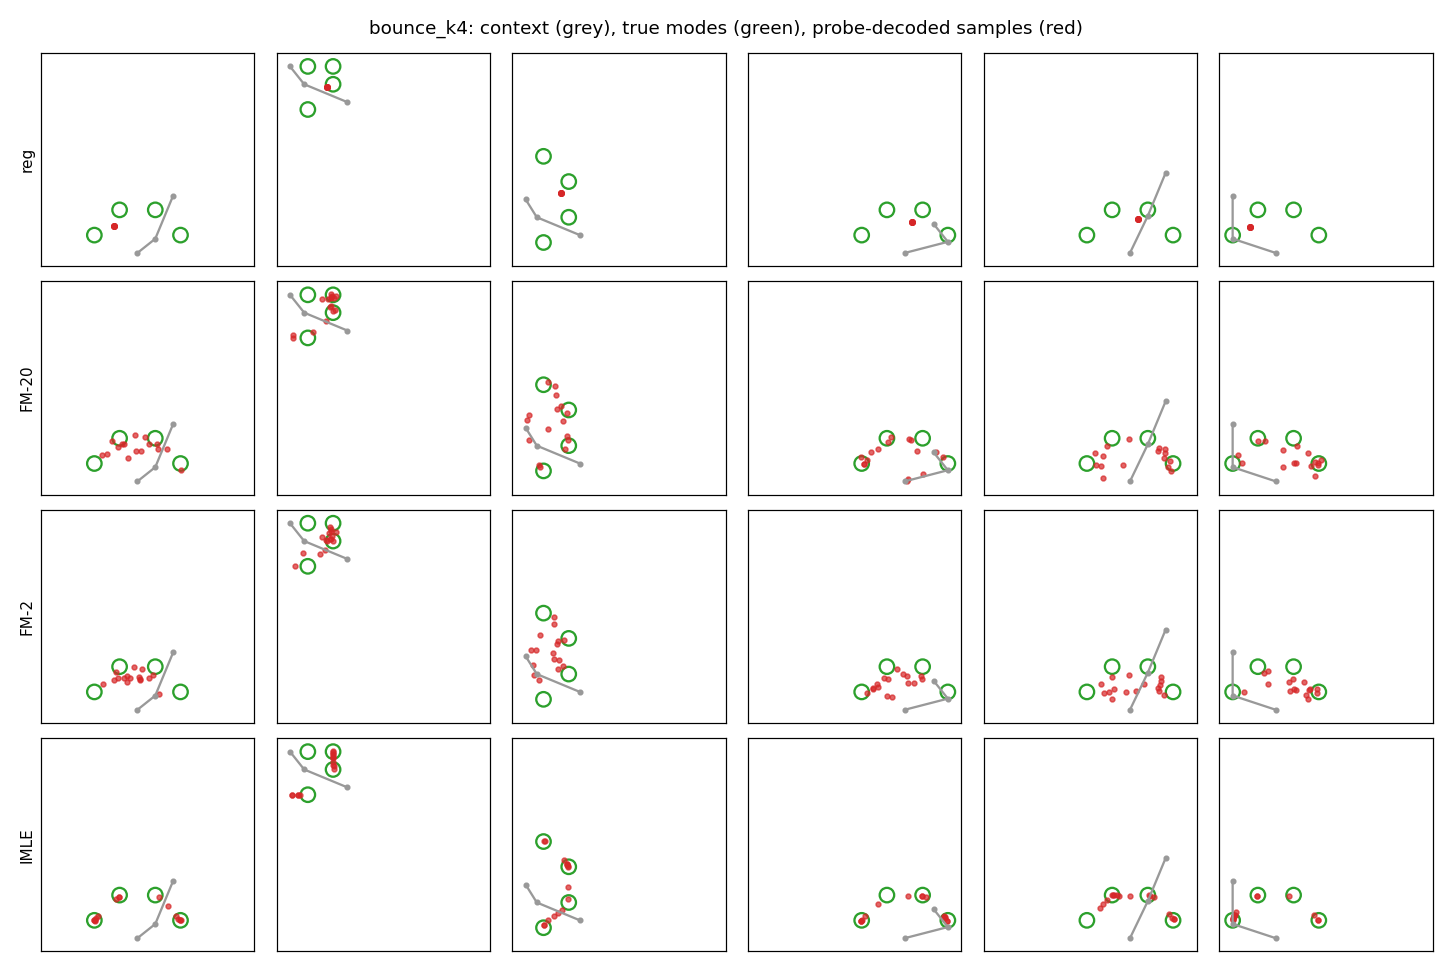
\includegraphics[width=\linewidth]{fig_scatter_pilot.png}
\caption{Qualitative pilot on the bounce environment with $K{=}4$ modes and fixed appearance (pilot recipe, $m{=}4$). Each column is one context whose ball has just hit a wall: gray, the three context frames; green circles, the four possible next positions; red, 16 samples decoded by the position readout. Regression (top) returns one point near the mean, flow matching with 20 or 2 Euler steps scatters between the modes, and \imlewm{} (pilot recipe) places its samples on the modes.}
\label{fig:scatter}
\end{figure}

\begin{figure}[h]
\centering
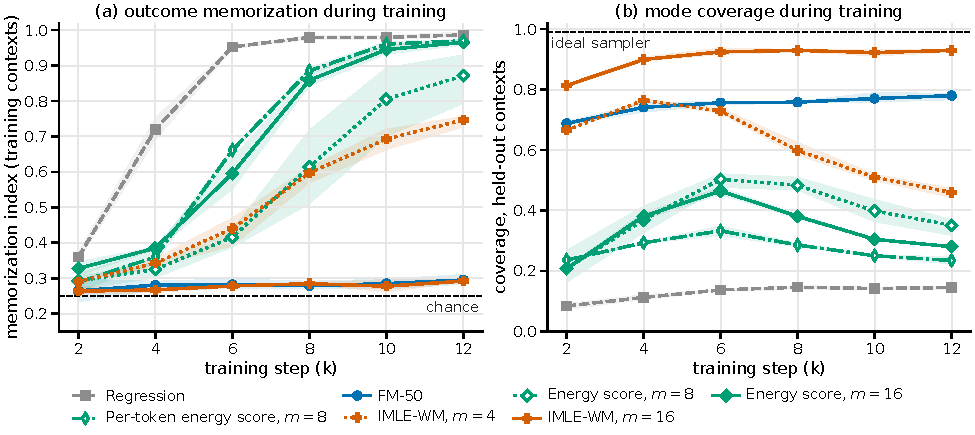
\includegraphics[width=\linewidth]{fig_memo_curves.pdf}
\caption{Memorization during training on A2-div ($K{=}4$; mean of three seeds, two for the energy score with $m{=}16$ and the per-token variant; band: min--max over seeds). (a) Memorization index on training contexts (dashed: chance $0.25$); on held-out contexts the seed means of every method stay between $0.22$ and $0.30$ (not shown). (b) Coverage on held-out contexts (dashed: ideal 16-sample sampler). Both panels come from the training monitor, which samples FM-50 with 20 Euler steps. Regression memorizes completely; \imlewm{} with $m{=}4$ and the three energy-score runs memorize progressively and lose coverage as they do; \imlewm{} with $m{=}16$ and FM-50 do not memorize within 12k steps.}
\label{fig:curves}
\end{figure}

\begin{table}[h]
\caption{Budget grid on A2-div at 8k steps, two seeds: memorization index (chance $1/K$), coverage, precision and deterministic-transition error (px). Coverage is capped by the ideal 16-sample sampler ($1.00$, $0.99$, $0.88$, $0.64$ for $K = 2, 4, 8, 16$). $K{=}16$ is under-trained at 8k steps: its kNN recall rises from $0.12$ to $0.85$ with $m$ while its coverage stays near $0.28$.}
\label{tab:grid}
\begin{center}
\small
\setlength{\tabcolsep}{4pt}
\begin{tabular}{lccccccccccccc}
\toprule
 & \multicolumn{4}{c}{$K{=}2$} & \multicolumn{4}{c}{$K{=}4$} & \multicolumn{4}{c}{$K{=}8$} \\
\cmidrule(lr){2-5}\cmidrule(lr){6-9}\cmidrule(lr){10-13}
$m$ & 2 & 4 & 8 & 16 & 4 & 8 & 16 & 32 & 4 & 8 & 16 & 32 \\
\midrule
Memo.\ index & 0.96 & 0.57 & 0.53 & 0.52 & 0.50 & 0.31 & 0.27 & 0.26 & 0.31 & 0.20 & 0.15 & 0.14 \\
Coverage & 0.66 & 0.92 & 0.97 & 0.99 & 0.65 & 0.89 & 0.92 & 0.90 & 0.41 & 0.58 & 0.64 & 0.62 \\
Precision & 0.78 & 0.85 & 0.85 & 0.68 & 0.69 & 0.76 & 0.77 & 0.72 & 0.54 & 0.62 & 0.64 & 0.60 \\
Det.\ err.\ (px) & 0.99 & 1.47 & 2.64 & 4.01 & 1.23 & 1.70 & 2.91 & 3.46 & 1.20 & 1.46 & 1.64 & 2.78 \\
\midrule
 & \multicolumn{5}{c}{$K{=}16$} \\
\cmidrule(lr){2-6}
$m$ & 4 & 8 & 16 & 32 & 64 \\
\cmidrule(lr){1-6}
Memo.\ index & 0.22 & 0.14 & 0.12 & 0.11 & 0.08 \\
Coverage & 0.17 & 0.25 & 0.28 & 0.27 & 0.25 \\
Precision & 0.32 & 0.38 & 0.41 & 0.38 & 0.33 \\
Det.\ err.\ (px) & 1.13 & 1.40 & 1.76 & 2.92 & 5.71 \\
\bottomrule
\end{tabular}
\end{center}
\end{table}

\begin{figure}[h]
\centering
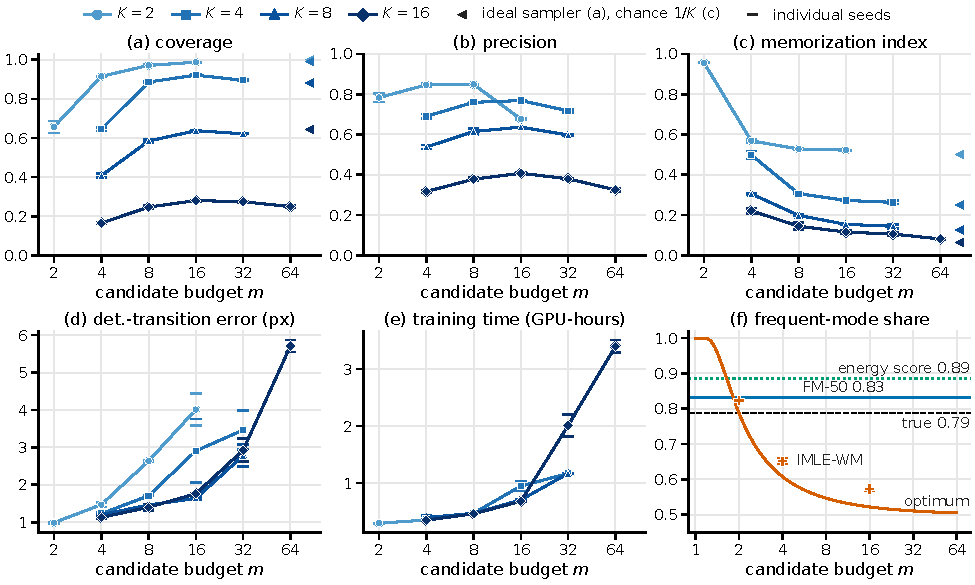
\includegraphics[width=\linewidth]{fig_m_knob.pdf}
\caption{Full version of Figure~\ref{fig:knob} (A2-div, 8k steps; markers: mean of two seeds, ticks: the seeds; triangles: ideal 16-sample sampler in (a), chance $1/K$ in (c)): (a) coverage, (b) precision, (c) memorization index, (d) deterministic-transition error, (e) training time (GPU-hours for 8k steps; some $K{=}16$ runs with large $m$ shared a GPU, which inflates their times) and (f) the raw frequent-mode share on the asymmetric variant ($K{=}2$; dashed: true share; curve: optimum of \citet{bennett2026freedom}), all against the budget $m$. The raw shares in (f) include the readout offset that Figure~\ref{fig:knob}d removes by subtracting the FM-50 share.}
\label{fig:knobfull}
\end{figure}

\begin{table}[h]
\caption{Countermeasures against outcome memorization on A2-div ($K{=}4$, 12k steps, two seeds; the $m{=}4$ and $m{=}16$ rows are the three-seed values of Table~\ref{tab:a2}). Memorization index for training / held-out contexts. Bold: best coverage, precision and kNN recall.}
\label{tab:counter}
\begin{center}
\small
\resizebox{\linewidth}{!}{%
\begin{tabular}{lcccccc}
\toprule
Variant & Coverage & Precision & kNN recall & Memo.\ (train / held-out) & Det.\ err.\ (px) & Train (h) \\
\midrule
$m{=}4$ & 0.46 & 0.68 & 0.65 & 0.75 / 0.25 & 1.14 & 0.6 \\
$m{=}4$ + RS-IMLE rejection ($\epsilon{=}0.5$) & 0.46 & 0.69 & 0.65 & 0.74 / 0.25 & 1.17 & 0.5 \\
$m{=}4$ + context noise $\sigma{=}1.0$ & 0.74 & 0.61 & 0.86 & 0.27 / 0.24 & 1.92 & 0.5 \\
$m{=}8$ + context noise $\sigma{=}0.3$ & 0.88 & 0.77 & 0.92 & 0.32 / 0.22 & 1.65 & 0.7 \\
$m{=}16$ & \best{0.93} & \best{0.82} & \best{0.94} & 0.29 / 0.24 & 1.55 & 1.1 \\
\bottomrule
\end{tabular}}
\end{center}
\end{table}

\begin{table}[h]
\caption{Asymmetric bounce ($K{=}2$, $p = 0.787$ on the evaluation contexts, 8k steps, two seeds): share of the frequent mode among 64 samples per held-out context, its theoretical optimum, coverage of both modes, and the memorization index on training / held-out contexts. With unequal mode probabilities the index of a model that does not memorize is $\sum_k p_k q_k$ rather than $1/K$; the held-out value measures it. Before these runs we had recorded shares of $0.80$, $0.61$ and $0.52$ for \imlewm{} and about $0.80$ for flow matching, computed for the nominal $p = 0.8$ and without a tolerance; the Theory column uses the realized frequency $0.787$.}
\label{tab:flatten}
\begin{center}
\small
\resizebox{\linewidth}{!}{%
\begin{tabular}{lccccc}
\toprule
Method & Frequent-mode share & Theory & Share $-$ FM-50 (measured / theory) & Coverage & Memo.\ index (train / held-out) \\
\midrule
\imlewm{}, $m{=}2$ & 0.823 & 0.787 & $-0.01$ / $0.00$ & 0.75 & 0.93 / 0.70 \\
\imlewm{}, $m{=}4$ & 0.651 & 0.607 & $-0.18$ / $-0.18$ & 0.96 & 0.68 / 0.58 \\
\imlewm{}, $m{=}16$ & 0.573 & 0.522 & $-0.26$ / $-0.27$ & 0.99 & 0.56 / 0.54 \\
FM-50 & 0.832 & 0.787 & -- & 0.95 & 0.73 / 0.68 \\
FM-2 & 0.915 & -- & $+0.08$ / -- & 0.80 & 0.77 / 0.73 \\
Energy score, $m{=}8$ & 0.886 & 0.787 & $+0.05$ / $0.00$ & 0.58 & 0.91 / 0.72 \\
\bottomrule
\end{tabular}}
\end{center}
\end{table}

\begin{figure}[h]
\centering
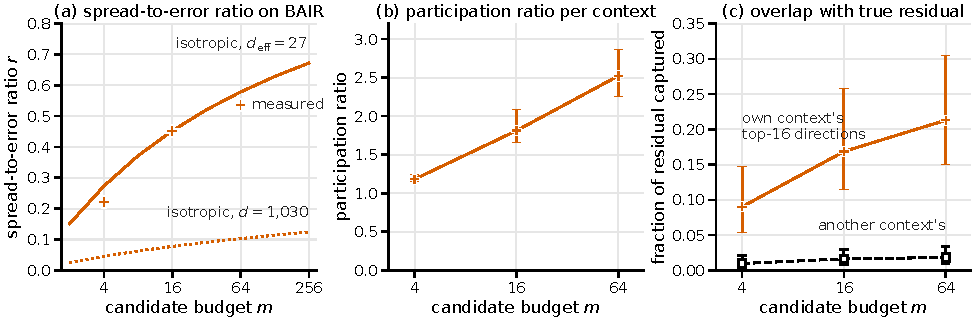
\includegraphics[width=\linewidth]{fig_bair.pdf}
\caption{Under-dispersion on BAIR ($h{=}1$, 256 evaluation contexts). (a) Spread-to-error ratio against $m$ (markers: measured, mean of two seeds that differ by less than $0.003$; one seed at $m{=}64$): the isotropic model of Proposition~\ref{prop:shrink} with one parameter fitted at $m{=}16$ ($\deff \approx 27$, solid) reproduces the $m{=}4$ and $64$ points within about $0.05$; with $d$ set to the measured participation ratio (PR) of the regression residuals ($\approx 1{,}030$, dotted) it predicts a spread five times too small; the PR of a covariance $S$ is $(\mathrm{tr}\,S)^2/\mathrm{tr}\,S^2$. (b), (c): seed 0; markers and bars: median and quartiles over the 256 contexts. (b) Participation ratio of the 64 samples of a context: one to three directions. (c) Fraction of the true residual in a context's own top-16 sample directions versus another context's: the directions are context-specific and aligned with the truth, but capture $9$--$21\%$ of it.}
\label{fig:bair}
\end{figure}

\begin{table}[h]
\caption{BAIR robot pushing, 21M models, two seeds (the $m{=}64$ and coarse-matching rows are one seed). Token RMS error of the best of 16 samples and of their mean, manifold distance and spread at $h{=}16$, Fr\'echet distance (FD) and kNN recall of mean-pooled PCA-32 tokens against 1{,}024 real frames. Bold: best two-seed row per column.}
\label{tab:bair}
\begin{center}
\small
\setlength{\tabcolsep}{3pt}
\resizebox{\linewidth}{!}{%
\begin{tabular}{lccccccccc}
\toprule
Method & NFE & \multicolumn{3}{c}{best-of-16 $\downarrow$ ($h{=}1/8/16$)} & mean $h{=}16$ $\downarrow$ & manifold $h{=}16$ $\downarrow$ & spread $h{=}16$ & FD $h{=}8/16$ $\downarrow$ & recall $h{=}8/16$ $\uparrow$ \\
\midrule
Regression & 1 & 0.268 & 0.481 & 0.556 & \best{0.556} & \best{1.27} & 0 & 1.44 / 2.65 & 0.21 / 0.08 \\
FM-50 & 50 & 0.338 & 0.681 & 0.843 & 0.885 & 1.78 & 0.94 & \best{0.53 / 1.38} & \best{0.73 / 0.84} \\
FM-2 & 2 & 0.302 & 0.590 & 0.734 & 0.756 & 1.45 & 0.72 & 1.42 / 2.75 & 0.26 / 0.08 \\
Shortcut & 1 & 0.401 & 0.902 & 1.173 & 1.197 & 1.71 & 1.48 & 0.95 / 1.77 & 0.42 / 0.26 \\
\imlewm{}, $m{=}4$ & 1 & 0.260 & 0.460 & 0.532 & 0.559 & 1.28 & 0.18 & 1.35 / 2.35 & 0.24 / 0.12 \\
\imlewm{}, $m{=}16$ & 1 & \best{0.258} & \best{0.456} & \best{0.527} & 0.576 & 1.30 & 0.29 & 1.22 / 2.09 & 0.28 / 0.15 \\
\imlewm{}, $m{=}64$ & 1 & 0.257 & 0.461 & 0.534 & 0.589 & 1.33 & 0.32 & 1.23 / 2.00 & 0.28 / 0.14 \\
\imlewm{}, $m{=}16$, coarse matching & 1 & 0.259 & 0.463 & 0.535 & 0.565 & 1.29 & 0.21 & 1.21 / 2.03 & 0.33 / 0.15 \\
\bottomrule
\end{tabular}}
\end{center}
\end{table}

\paragraph{Memorization with longer training and larger models (pilot recipe, A2-div, $K{=}4$, one seed).} With $m{=}4$, doubling the training steps (12k $\to$ 24k) raised the memorization index from $0.66$ to $0.92$ and lowered held-out coverage from $0.52$ to $0.38$; a $2.8\times$ larger model (19M) at 12k steps reached $0.86$ with coverage $0.43$. On held-out contexts the index stayed at chance ($0.23$--$0.25$) in all three runs. With $m{=}16$, training $1.5\times$ longer left the index at $0.31$ (Appendix~\ref{app:impl}).

\paragraph{Baseline fairness checks.}
iMF: a 72k-step run on A2-div (one seed, checkpoints every 6k steps) saturates after 24k steps at coverage $0.56$--$0.58$ and precision $0.24$--$0.26$, so its 36k training steps in the main tables are not the limiting factor. Flow matching: with four times the steps on A1 (48k, one seed) the F1 error becomes $4.08$ (\imlewm{} $m{=}4$), $7.10$ (FM-2) and $8.99$ (FM-50) under the probe, and $4.20$ for \imlewm{} under the heatmap readout; the FlowWM recipe (wide head, time shift 13, 50 steps) raised the A2-div coverage of our initial 20-step flow baseline from $0.58$ to $0.79$ and its precision from $0.38$ to $0.51$. Shortcut: trained for 24k steps so that its wall-clock time ($0.7$\,h on A2, $1.5$\,h on B) is below that of \imlewm{} with $m{=}16$; sampling with two steps instead of one changed its coverage and precision by less than $0.01$. Parameter counts: $7.97$--$8.24$M (8M setting), $20.6$M (21M setting).


\FloatBarrier
\subsection{Rollout metrics}
\begin{figure}[h]
\centering
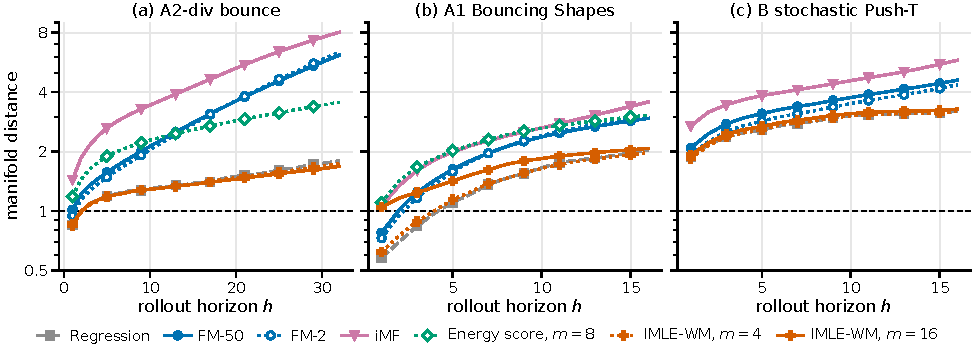
\includegraphics[width=\linewidth]{fig_manifold.pdf}
\caption{Manifold distance of autoregressive rollouts against the horizon (16 rollouts from each of 128 real contexts; mean of three seeds, two for the energy score on A1 and for iMF on B; shared logarithmic $y$-axis; dashed line: $1$ = on the data). \imlewm{} with $m{=}4$ stays as close to the data as regression on all three benchmarks, and $m{=}16$ does so on A2-div and Push-T; on Bouncing Shapes $m{=}16$ starts higher ($1.05$ vs.\ $0.58$ at $h{=}1$) and meets regression at $h{=}16$. Flow-matching rollouts drift equally with 50 and with 2 integration steps, and iMF drifts most. The energy score ($m{=}8$) starts above flow matching on A2-div and drifts less from $h \approx 13$ on ($3.6$ vs.\ $6.2$ at $h{=}32$). Shortcut rollouts were not evaluated.}
\label{fig:manifold}
\end{figure}
Table~\ref{tab:e3} completes Figure~\ref{fig:manifold} with the best-of-16 readout error and the spread at the last horizon.

\begin{table}[h]
\caption{Rollouts from real contexts (16 samples, three seeds; iMF on Push-T two): manifold distance, best-of-16 readout error (px) and spread (px; mean distance over pairs of distinct rollouts) at the last horizon ($h{=}32$ on A2-div, $16$ on A1 and B). Bold: lowest manifold distance and best-of-16 error per benchmark.}
\label{tab:e3}
\begin{center}
\small
\setlength{\tabcolsep}{4pt}
\begin{tabular}{lccccccccc}
\toprule
 & \multicolumn{3}{c}{A2-div, $h{=}32$} & \multicolumn{3}{c}{A1 Bouncing Shapes, $h{=}16$} & \multicolumn{3}{c}{B Push-T, $h{=}16$} \\
\cmidrule(lr){2-4}\cmidrule(lr){5-7}\cmidrule(lr){8-10}
Method & manifold & best-of-16 & spread & manifold & best-of-16 & spread & manifold & best-of-16 & spread \\
\midrule
Regression & 1.80 & 32.2 & 0 & 2.04 & 34.0 & 0 & 3.21 & 102.2 & 0 \\
FM-50 & 6.16 & 9.8 & 27.4 & 2.95 & 28.0 & 26.8 & 4.60 & \best{67.4} & 38.9 \\
FM-2 & 6.36 & 10.6 & 28.6 & 3.03 & 23.4 & 27.8 & 4.37 & 69.2 & 31.6 \\
iMF & 8.04 & 10.1 & 30.9 & 3.57 & 33.4 & 36.1 & 5.81 & 84.1 & 60.8 \\
\imlewm{}, $m{=}4$ & 1.74 & 10.5 & 25.5 & \best{1.98} & \best{19.0} & 15.9 & \best{3.20} & 88.7 & 9.9 \\
\imlewm{}, $m{=}16$ & \best{1.68} & \best{9.3} & 29.0 & 2.08 & 19.4 & 19.1 & 3.28 & 79.1 & 23.3 \\
\bottomrule
\end{tabular}
\end{center}
\end{table}

\FloatBarrier
\subsection{Stochastic Push-T: bootstrap intervals}
Table~\ref{tab:bci} gives the paired differences behind Section~\ref{sec:b} and Section~\ref{sec:seq}. No model resolves the four modes of this benchmark: with the tolerance rule of the coverage metric (capped at $20$\,px here), the mode coverage at $h{=}16$ is at most $0.03$ for every model and seed in Table~\ref{tab:b}, and $0.06$--$0.08$ with per-step matching.

\begin{table}[h]
\caption{Paired differences on the stochastic Push-T multi-future test set (px; negative favors the first model) with 95\% bootstrap confidence intervals (CI) over the 128 starting states after averaging seeds, and hierarchical intervals that also resample the three seeds (10{,}000 resamples). The $h{=}8$ rows use the first 8 steps of the 16-step rollouts, so they differ slightly from the separate 8-step evaluation of Table~\ref{tab:b}.}
\label{tab:bci}
\begin{center}
\small
\begin{tabular}{llcccc}
\toprule
Comparison & Metric & Difference & Start-state CI & Hierarchical CI \\
\midrule
\imlewm{} 16 vs.\ FM-50 & $h{=}8$ recall error & $-1.8$ & $[-2.5, -1.1]$ & $[-5.2, +2.3]$ \\
 & $h{=}8$ precision error & $-5.2$ & $[-5.7, -4.8]$ & $[-8.0, -2.5]$ \\
 & $h{=}16$ recall error & $-4.2$ & $[-5.3, -3.1]$ & $[-8.8, +1.1]$ \\
 & $h{=}16$ precision error & $-6.6$ & $[-7.6, -5.7]$ & $[-8.5, -4.7]$ \\
\imlewm{} 16 vs.\ FM-2 & $h{=}16$ recall error & $-3.7$ & $[-4.9, -2.5]$ & $[-8.7, +1.9]$ \\
 & $h{=}16$ precision error & $-5.6$ & $[-6.6, -4.6]$ & $[-7.7, -3.2]$ \\
\imlewm{} 16 vs.\ Shortcut & $h{=}16$ recall error & $-8.2$ & $[-10.0, -6.3]$ & $[-11.3, -4.0]$ \\
 & $h{=}16$ precision error & $-13.2$ & $[-15.1, -11.3]$ & $[-16.3, -10.2]$ \\
Per-step vs.\ one-step matching (8k) & $h{=}8$ recall error & $-7.1$ & $[-8.2, -6.0]$ & $[-9.2, -4.8]$ \\
 & $h{=}16$ recall error & $-14.3$ & $[-16.3, -12.5]$ & $[-19.1, -9.9]$ \\
 & $h{=}16$ precision error & $-17.0$ & $[-18.4, -15.6]$ & $[-20.4, -14.5]$ \\
\bottomrule
\end{tabular}
\end{center}
\end{table}

\FloatBarrier
\subsection{Energy-score follow-ups}
\label{app:es}
\begin{table}[h]
\caption{Energy score against \nom{} on bounce (12k steps; two seeds unless noted). A2-div: randomized appearance, contexts never repeat. A2-fix: fixed appearance, no identifying key (same recipe for all rows). The manifold distance at $h{=}1$ is in units of the median real-to-real distance (A2-fix: relative to \imlewm{} $m{=}16$). A1 and the readout comparison are in Appendix~\ref{app:readout}. Bold: best coverage, precision and kNN recall within each setting.}
\label{tab:es}
\begin{center}
\footnotesize
\setlength{\tabcolsep}{4pt}
\begin{tabular}{llcccccc}
\toprule
Setting & Method & Coverage & Precision & kNN recall & Memo.\ index & Det.\ err.\ (px) & Manifold $h{=}1$ \\
\midrule
A2-div & Energy score, $m{=}8$ (3 seeds) & 0.36 & 0.61 & 0.77 & 0.87 & 1.06 & 1.19 \\
 & Energy score, $m{=}16$ & 0.28 & 0.61 & 0.60 & 0.97 & 1.06 & 1.16 \\
 & Per-token energy score, $m{=}8$ & 0.22 & 0.55 & 0.44 & 0.97 & 1.33 & 1.12 \\
 & \imlewm{}, $m{=}4$ (3 seeds) & 0.46 & 0.68 & 0.65 & 0.75 & 1.14 & 0.84 \\
 & \imlewm{}, $m{=}16$ (3 seeds) & \best{0.93} & \best{0.82} & \best{0.94} & 0.29 & 1.55 & 0.86 \\
\midrule
A2-fix & Energy score, $m{=}8$ & 0.95 & 0.81 & \best{1.00} & 0.27 & 0.20 & $1.59\times$ \\
 & \imlewm{}, $m{=}4$ & 0.97 & 0.91 & 0.68 & 0.26 & 0.15 & $0.94\times$ \\
 & \imlewm{}, $m{=}16$ & \best{0.99} & \best{0.95} & 0.85 & 0.25 & 0.91 & $1\times$ \\
\bottomrule
\end{tabular}
\end{center}
\end{table}
Figure~\ref{fig:toy} shows the toy experiment of Section~\ref{sec:es}. The task is the two-branch problem of \citet{makabe2026esp} ($u \sim U[0.05, 1]$, $y = \pm\sqrt{u} + 0.08\varepsilon$, equiprobable modes) with a 16-dimensional nuisance vector $a \sim \mathcal{N}(0, I)$ appended to the context, a three-layer MLP generator of width 256 with a 4-dimensional noise input, Adam at $2\times10^{-4}$, batch 256, 15k steps, and the same energy-score estimator as the main runs. With fresh contexts at every step the energy score matches $0.940$ / $0.946$ of its samples to a mode center within $0.24$ ($m = 8$ / $16$) and \nom{} $0.916$ / $0.924$. With 1{,}024 fixed training contexts (about 3{,}750 revisits each) the energy score memorizes (index $0.999$) and covers both modes on $0.2\%$ of new contexts, while \nom{} with $m = 8$ / $16$ is at $0.52$ / $0.51$ and covers $0.99$ / $1.00$. With 4{,}096, 16{,}384 and 65{,}536 contexts the energy score's memorization index is $0.73$, $0.51$ and $0.50$; without the nuisance vector (context $= u$ only) it is $0.50$ even with 1{,}024 contexts (one seed each). The thresholds are those of this small network and do not transfer; the 8M model on A2-div saw each of its $11{,}559$ stochastic training contexts about 38 times and memorized.

\begin{figure}[h]
\centering
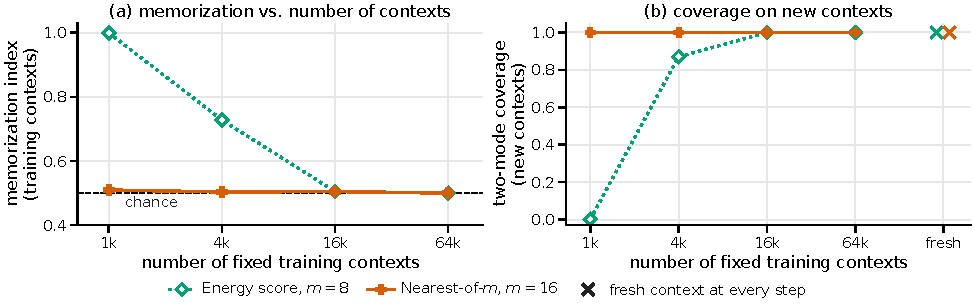
\includegraphics[width=\linewidth]{fig_toy.pdf}
\caption{Toy two-branch problem with a 16-dimensional nuisance appearance vector ($m{=}8$ for the energy score and $16$ for \nom{}; two seeds for fresh contexts and for 1{,}024 contexts, which agree within $0.01$; one seed for 4{,}096 or more). (a) Memorization index on training contexts against the number of fixed training contexts (fewer contexts mean more revisits of each; dashed: chance $0.5$). (b) Fraction of new contexts on which both modes are covered; crosses: a fresh context at every training step (both methods reach $1.00$; drawn side by side).}
\label{fig:toy}
\end{figure}

The follow-up runs on A2-fix and with the per-token score were preceded by five recorded predictions, all of which held (two seeds each): (P1) the energy score with $m{=}8$ does not memorize on A2-fix (index $\le 0.40$; observed $0.268$); (P2) its coverage on A2-fix exceeds its A2-div value but stays below \imlewm{} with $m{=}16$ in both coverage and precision (observed $0.947$ vs.\ $0.987$ and $0.814$ vs.\ $0.954$); (P3) \imlewm{} with $m{=}4$ does not memorize on A2-fix ($\le 0.35$; observed $0.256$); (P4) the per-token energy score memorizes on A2-div (index $\ge 0.7$, coverage $\le 0.5$; observed $0.970$ and $0.224$); (P5) its manifold distance at $h{=}1$ exceeds $1.1$ (observed $1.12$; \imlewm{} $0.86$). On A2-fix the energy score's kNN recall is $1.00$ against $0.85$ for \imlewm{}, so its samples spread more widely than the outcomes; its deterministic-transition error is lower than that of \imlewm{} with $m{=}16$ ($0.20$ vs.\ $0.91$\,px). On A2-div its learning curves peak in coverage at 6k steps ($0.50$) and decline as the index rises ($0.42 \to 0.87$); the two $m{=}16$ seeds reach an index of $0.84$ and $0.87$ at 8k steps against $0.51$--$0.72$ for the three $m{=}8$ seeds. Token-space diagnostics at $h{=}1$ on A2-div (three seeds, evaluation contexts): spread-to-error ratio $0.80$ (energy score) vs.\ $0.64$ (\imlewm{} 16), $0.38$ (\imlewm{} 4), $1.15$ (FM-50); best-of-16 token error $0.468$ vs.\ $0.271$; mean-prediction error $0.451$ vs.\ $0.396$; readout spread $1.6$ vs.\ $4.1$\,px; manifold distance at $h{=}1$ $1.19$ vs.\ $0.86$.

\FloatBarrier
\subsection{Per-step matching}
\label{app:seq}

\begin{table}[h]
\caption{Per-step matching on self-rollouts ($H{=}4$) against one-step matching on stochastic Push-T at equal training steps (8k, but $3.9\times$ the wall-clock time; 21M, three seeds): precision / recall error (px) and the paired per-seed change; bold: lower error.}
\label{tab:seq}
\begin{center}
\scriptsize
\setlength{\tabcolsep}{5pt}
\begin{tabular}{lccc}
\toprule
Stochastic Push-T & $h{=}8$ prec.\ / recall err. & $h{=}16$ prec.\ / recall err. & Train (h) \\
\midrule
One-step matching & 25.7 / 25.4 & 41.6 / 43.7 & 1.3 \\
Per-step, feed matched & \best{18.8} / \best{18.4} & \best{24.6} / \best{29.3} & 5.3 \\
Paired change & $-27\%$ / $-28\%$ & $-41\%$ / $-33\%$ & $\times 3.9$ \\
One-step matching, 12k steps & 21.8 / 22.1 & 34.1 / 37.8 & 2.2 \\
\bottomrule
\end{tabular}
\end{center}
\end{table}

\begin{table}[h]
\caption{Fed-back-state ablation on Bouncing Shapes (8M, $m{=}16$, 8k steps, two seeds): manifold distance, best-of-16 readout error and spread of the 16 rollouts at $h{=}16$ (the true futures spread by $23.6$\,px), and F1 error. All three predictions recorded before the ablation held (S1--S3 below). Bold: best manifold distance and best-of-16 error; the F1 differences are within the seed variation.}
\label{tab:seqabl}
\begin{center}
\small
\begin{tabular}{lcccc}
\toprule
Fed-back state & Manifold & Best-of-16 & Spread & F1 \\
\midrule
One-step matching & 2.17 & 23.2 & 17.0 & 8.74 \\
Per-step, feed matched & 1.92 & \best{17.7} & 26.3 & 8.51 \\
Per-step, feed random candidate & \best{1.81} & 22.9 & 12.4 & 8.77 \\
Per-step, feed true frame & 2.14 & 23.6 & 16.6 & 8.62 \\
\bottomrule
\end{tabular}
\end{center}
\end{table}

\begin{figure}[h]
\centering
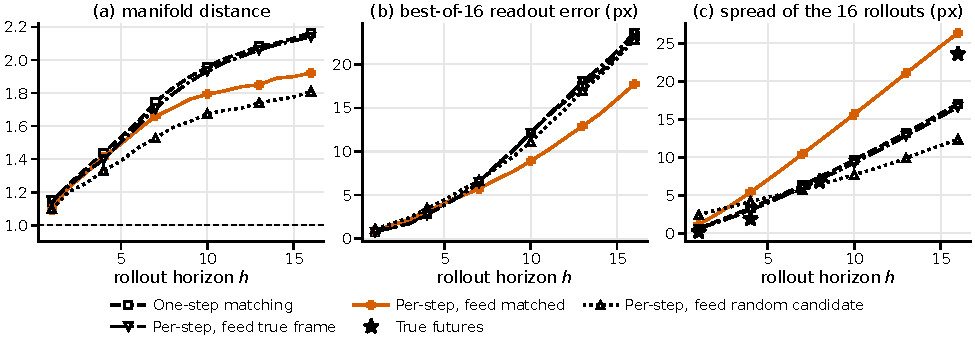
\includegraphics[width=\linewidth]{fig_seq_ablation.pdf}
\caption{The fed-back-state ablation on Bouncing Shapes (mean of two seeds). (a) Any self-generated context, matched or random, keeps the rollout closer to the manifold (dashed: $1$ = on the data); the true frame does not. (b) Only the candidate nearest the truth improves the best-of-16 error. (c) Spread of the 16 rollouts; stars: true futures. At $h{=}16$ only the matched variant reaches the true spread ($26.3$ vs.\ $23.6$\,px), but it over-spreads at $h \le 8$ ($12.2$ vs.\ $6.8$\,px at $h{=}8$); the random variant jitters at $h{=}1$ and ends at half the true spread.}
\label{fig:seqabl}
\end{figure}
Per-seed Push-T recall errors at $h{=}16$ (one-step $\to$ per-step): $43.7 \to 30.3$, $42.6 \to 32.2$, $44.7 \to 25.5$. On the deterministic Push-T control (one seed) the best-of-16 T-vertex error at $h = 4 / 8 / 16$ moves from $35.8 / 60.4 / 72.3$ to $29.2 / 45.6 / 58.9$\,px and the manifold distance at $h{=}16$ from $3.90$ to $3.64$. On A2-div (two seeds, 8k steps) the manifold distance at $h = 8 / 16 / 32$ moves from $1.31 / 1.47 / 1.83$ to $1.19 / 1.26 / 1.40$ while coverage and precision at $h{=}1$ move from $0.92 / 0.77$ to $0.90 / 0.73$ and the deterministic-transition error from $2.91$ to $3.97$\,px; the best-of-16 error is unchanged. On A1 (two seeds) F1 moves from $8.74$ to $8.51$ (precision error $9.26 \to 9.77$, recall error $8.28 \to 7.55$), the manifold distance at $h{=}16$ from $2.17$ to $1.92$ and the best-of-16 error from $23.2$ to $17.7$\,px. The fed-back-state ablation was preceded by three recorded predictions: (S1) feeding back the true frame yields less than half of the manifold gain (manifold at $h{=}16$ $\ge 2.05$; observed $2.14$); (S2) feeding back a random candidate yields more than half ($\le 2.05$; observed $1.81$); (S3) the random candidate's best-of-16 error exceeds the matched one's by at least $1$\,px ($\ge 18.7$; observed $22.9$). The spread of the 16 rollouts at $h = 1 / 4 / 8 / 16$ is $0.20 / 1.90 / 6.81 / 23.6$\,px for the true futures, $0.70 / 3.35 / 7.42 / 17.0$ for one-step matching, $1.16 / 5.42 / 12.2 / 26.3$ for the matched variant, $2.41 / 4.19 / 6.38 / 12.4$ for the random variant and $0.61 / 3.07 / 7.08 / 16.6$ for the true-frame variant. Training times: one-step $0.68$\,h, per-step variants $2.7$\,h (8M, 8k steps).

\FloatBarrier
\subsection{Planning details}
\label{app:plan}
\begin{table}[h]
\caption{Planning with CEM-MPC; mean $\pm$ s.d.\ over three seeds of 100 episodes (FM-50 on Push-T: one seed, 10 episodes). (a) Stochastic Push-T: success rate and wall-clock planning time per MPC step, amortized over a batch of 100 parallel episodes (FM-50: 10). (b) Branch-risk task: success, pit and timeout rates, and the model's estimate of the pit probability after one push on the ice (true $0.33$) and after five straight pushes from 200 start states (true $0.43$). FM-50 was evaluated for its risk estimates only. Bold: best learned planner in planning time, branch-risk success and pit rate.}
\label{tab:plan}
\vspace{4pt}\centering\footnotesize
\setlength{\tabcolsep}{3.5pt}
\begin{tabular}{@{}l cc c ccc cc@{}}
\toprule
 & \multicolumn{2}{c}{(a) Stochastic Push-T} & & \multicolumn{5}{c}{(b) Branch-risk task} \\
\cmidrule(lr){2-3}\cmidrule(l){5-9}
 & Success & Time & & Success & Pit & Timeout & \multicolumn{2}{c}{Estimated pit probability} \\
Model & (\%) $\uparrow$ & (s/step) $\downarrow$ & & (\%) $\uparrow$ & (\%) $\downarrow$ & (\%) & 1 push (0.33) & 5 pushes (0.43) \\
\midrule
Oracle (true simulator) & --             & --         & & 76             & 7              & 17   & 0.33           & 0.43 \\
Regression              & \sd{31.7}{3.3} & 4.3        & & \sd{56.3}{3.4} & \sd{24.3}{2.5} & 19.3 & \sd{0.61}{.10} & \sd{0.26}{.19} \\
FM-2                    & \sd{34.7}{3.1} & 8.5        & & \best{\sd{67.0}{1.4}} & \best{\sd{18.7}{0.9}} & 14.3 & \sd{0.14}{.00} & \sd{0.38}{.06} \\
FM-50                   & 30             & 200        & & --             & --             & --   & \sd{0.31}{.02} & 0.44 \\
\imlewm{}, $m{=}16$     & \sd{31.7}{2.1} & \best{4.0} & & \sd{55.3}{2.6} & \sd{31.0}{2.2} & 13.7 & \sd{0.36}{.03} & \sd{0.44}{.04} \\
\bottomrule
\end{tabular}
\end{table}
On stochastic Push-T the final block position and angle errors are $46.6$\,px / $42.0^\circ$ (regression), $40.6$ / $35.2$ (FM-2), $45.2$ / $20.0$ (FM-50, 10 episodes) and $49.5$ / $44.9$ (\imlewm{}). The contact error of a single transition (block displacement after a contact transition, true $15.9$\,px) is $11.7$ / $11.2$\,px for regression at 12k / 36k steps, $12.4$ / $12.6$ for FM-2 / FM-50 and $12.2$ / $12.3$ for \imlewm{} with $m = 4$ / $16$ (seed 0). On the branch-risk task the per-start absolute error of the five-push pit probability is $0.078$ (\imlewm{}), $0.086$ (FM-50), $0.096$ (FM-2) and $0.462$ (regression), and the timeout rates are $13.7\%$ (\imlewm{}), $14.3\%$ (FM-2), $19.3\%$ (regression) and $17\%$ (oracle). Wall-clock for 100 episodes: oracle $100$\,s, regression $523$\,s ($m_p{=}1$), \imlewm{} $3{,}633$\,s, FM-2 $9{,}067$\,s.

\FloatBarrier
\section{Negative results}
\label{app:negative}
The first four paragraphs below describe additions that the pilot study tested and the final recipe does not use; the last one collects two BAIR variants that did not help either.

\paragraph{Trajectory-level matching.}
Matching $m{=}4$ candidate rollouts of length $H{=}8$ as whole trajectories (with a curriculum $H = 1 \to 4 \to 8$) on the push environment was worse than one-step matching at every horizon: best-of-16 position error $1.31$ vs.\ $0.35$\,px at $h{=}1$, $3.89$ vs.\ $2.19$ at $h{=}8$, $4.67$ vs.\ $3.03$ at $h{=}16$ (paired bootstrap intervals exclude zero), coverage at $h{=}1$ of $0.71$ vs.\ $0.98$, and $3.3\times$ the training time; only the error of the sample mean improved ($9.18$ vs.\ $9.94$ at $h{=}16$), the signature of averaging. With two to three modes per step an 8-step trajectory has hundreds of trajectory modes, far beyond $m{=}4$, so the matched candidate is the one close to all of them on average. Per-step matching (Section~\ref{sec:seqmatch}) replaced it.

\paragraph{Multi-stage supervision.}
On the fixed $16\times16$ token grid, supervising intermediate heads with spatially pooled targets ($4\times4$, $8\times8$, $16\times16$) or with PCA-truncated targets (32, 128, 384 components) gave the same coverage as a single head within the bootstrap interval ($0.960$ and $0.959$ vs.\ $0.967$ at $K{=}4$) and the same precision ($0.916$, $0.922$ vs.\ $0.926$). The final recipe uses a single head.

\paragraph{Variance-penalized planning.}
A CEM cost of mean plus $\lambda$ times the spread of the imagined goal distances lowered the success rate of the branch-risk task even when the true simulator served as the world model: $78\%$, $77\%$, $70\%$ and $50\%$ at $\lambda = 0, 0.5, 1, 2$ (60 episodes; the 100-episode run of Table~\ref{tab:plan} gives $76\%$ at $\lambda = 0$), with the pit rate rising to $35\%$. A certain failure has zero variance, so the penalty prefers it to an uncertain success. With \imlewm{} as the model (two task seeds, 60 episodes each) the pooled success was $62.5\%$ at $\lambda = 0$ and $61.7\%$ at $\lambda = 0.5$.

\paragraph{Counterfactual action contrast.}
We had anticipated that the noise $z$ might absorb the effect of the action. It does not: on the push environment the counterfactual precision (the fraction of samples under a random other action that land on the enumerated outcomes of that action) and the action sensitivity (the change in output per change in action, relative to the true change) are $0.95$ and $0.96$ with the action on its own FiLM path, $0.92$ and $0.97$ with the action merged into the noise path, and $0.93$ and $0.975$ with an added margin term, against $0.83$ and $0.94$ for regression. There was no shortcut to repair.

\paragraph{Low-dimensional matching and larger budgets on BAIR.}
See Table~\ref{tab:bair}: over $h = 1$ to $16$, $m{=}64$ raises the spread-to-error ratio from $0.43$--$0.51$ to $0.51$--$0.56$ ($0.45$ and $0.54$ at $h{=}1$) at $2.4\times$ the training time, and matching in a 512-dimensional pooled space lowers it to $0.31$--$0.39$ ($0.32$ at $h{=}1$); neither approaches FM-50 on distribution metrics.

\FloatBarrier
\section{Statistical methodology}
\label{app:stats}
Per-context intervals are percentile bootstrap intervals (2{,}000 resamples) over the 400 evaluation contexts of a run, used in the pilot and recipe tables. Seed statistics are means and standard deviations over the listed seeds; the $\pm$ values in the tables are these standard deviations, computed with the $1/n$ normalization. For the Push-T multi-future test set, each model's per-start errors were stored; the start-state interval averages the seeds first and resamples the 128 starts, and the hierarchical interval resamples the seeds with replacement and then the starts, 10{,}000 times each. Per-step and one-step matching runs with the same seed are paired. All comparisons report the direction and the magnitude of the difference; where an interval includes zero we say so in the text.
